\def\year{2017}\relax
%File: formatting-instruction.tex
\documentclass[letterpaper]{article}
\usepackage{aaai17}
\usepackage{times}
\usepackage{helvet}
\usepackage{courier}
\frenchspacing
\setlength{\pdfpagewidth}{8.5in}
\setlength{\pdfpageheight}{11in}
\usepackage{cite}
\usepackage{subcaption}
\usepackage{hyperref}
\usepackage{mathtools}
\usepackage{amssymb}

\usepackage{graphicx}

\usepackage{titling}
\graphicspath{{figures/final/}}


\pdfinfo{
/Title (Shaping Model-Free Reinforcement Learning with Model-Based Pseudorewards)}
\setcounter{secnumdepth}{0}  
 \begin{document}
% The file aaai.sty is the style file for AAAI Press 
% proceedings, working notes, and technical reports.
%

\title{Shaping Model-Free Reinforcement Learning with Model-Based Pseudorewards}
\date{}
\maketitle
\begin{abstract}
Model-free and model-based reinforcement learning have provided a successful framework for understanding both human behavior and neural data. These two systems are usually thought to compete for control of behavior. However, it has also been proposed that they can be integrated in a cooperative manner. For example, the Dyna algorithm uses model-based replay of past experience to train the model-free system, and has inspired research examining whether human learners do something similar. Here we introduce an approach that links model-free and model-based learning in a new way: via the reward function. Given a model of the learning environment, dynamic programming is used to iteratively estimate state values that monotonically converge to the state values under the optimal policy. Pseudorewards are calculated from these values and used to shape the reward function of a model-free learner in a way that is guaranteed not to change the optimal policy. In two experiments we show that this method offers computational advantages over Dyna. It also offers a new way to think about integrating model-free and model-based reinforcement learning: that our knowledge of the world doesn't just provide a source of simulated experience for training our instincts, but that it shapes the rewards that those instincts latch onto.
%One interesting hypothesis is that emotions may in certain conditions function as model-based pseudorewards that tune a model-free system.
\end{abstract}

\section{Introduction}

The problem of learning from environmental rewards has been studied extensively in both psychology and artificial intelligence research. Both fields have explored two different approaches to solving this problem, known as model-free and model-based reinforcement learning. Model-free learning relies on direct trial-and-error interaction with the environment~\cite{sutton1992reinforcement}, while model-based learning leverages knowledge about the causal structure of the environment~\cite{barto1995learning}. Historically, animal psychologists viewed these two systems as distinct and competing hypotheses, with behaviorists arguing in favor of reflexive, model-free learning based on stimulus-response associations~\cite{thorndike1933proof}, and Tolman and others positing an internal representation of the environment, known as the ``cognitive map"~\cite{tolman1948cognitive}.

Nowadays, while both behavioral and neural data indicate that human learning relies on both systems~\cite{daw2005uncertainty, glascher2010states, dayan2014model}, it is typically assumed that they only compete for control of behavior. However, it is also possible for both systems to cooperate. The Dyna architecture achieves such cooperation by integrating model-free learning with model-based planning~\cite{sutton1991dyna}. In Dyna, as model-free learning occurs, transitions between states of the environment and the resulting rewards are stored in a model. That model is used to replay these past experiences, using them to further train model-free state-action values. Recent behavioral data from people performing a retrospective revaluation task is consistent with a cooperative architecture like Dyna~\cite{gershman2014retrospective}.

Here we introduce a new method for cooperative interaction between model-free and model-based learning. The model-based system generates pseudorewards that are used to shape the reward function used in model-free learning. According to the \textit{shaping theorem}, conditions exist under which the optimal decision policy will remain invariant to such modifications of the reward function, opening the possibility that pseudorewards can be used to guide agents toward optimal behavior~\cite{ng1999policy}. That is, if the optimal policy can be guaranteed to remain unchanged with the introduction of pseudorewards, then pseudorewards can potentially be used to guide the agent to the optimal policy. Using these principles, we show that pseudorewards can be used to link model-free and model-based learning through modification of the reward function.

This method of cooperation between learning systems offers an appealing alternative to Dyna both conceptually and practically. The model-based replay of past experience used to refine state-action values in Dyna suggests that planning (by internal simulation) is one way that different learning systems might be linked in human cognition. The method that we introduce offers an alternative approach, based on changing the reward function. One way that this link may manifest in human cognition is through model-based production of emotions that function as pseudorewards for model-free learning. In addition to providing a new way to think about interaction between reinforcement learning systems, our method also offers a practical advantages over Dyna by learning in fewer steps and requiring less computation time.

We begin by reviewing the Dyna architecture for integrated model-free and model-based learning. We then introduce our method and the theoretical background on which it is based. We present two experiments which show the effectiveness of ourmethod, and how it compares to Dyna. The first experiment involves learning in a maze environment, and the second experiment uses the classic mountain car problem. We end by discussing additional variants of Dyna and our method, and consider how this integrated approach might provide a useful model for understanding human cognition and emotion.

\section{Cooperative Reinforcement Learning}

\subsection{Markov Decision Processes}

We describe sequential decision problems that can be modeled as a \textit{Markov Decision Process (MDP)}. The MDP is defined as the 5-tuple: $M=\{\mathcal{S},\mathcal{A},\mathcal{P},\mathcal{R},\gamma\}$, where $\mathcal{S}$ is the set of states, $\mathcal{A}$ is the set of actions, and for each $(s,a) \in \mathcal{S} \times \mathcal{A}$, $\mathcal{P}(s,a,s')$ is the probability of transitioning to state $s'$ when action $a$ is selected in state $s$, $\mathcal{R}(s,s')$ is the reward received for transitioning from state $s$ to $s'$, and $\gamma^t$ is the discount factor for rewards $t$ time steps in the future, where $0\leq\gamma\leq1$~\cite{sutton1998reinforcement}. A \textit{policy}, $\pi$, is a mapping of states, $\mathcal{S}$, onto actions, $\mathcal{A}$: $\pi:\mathcal{S}\mapsto\mathcal{A}$. A \textit{value function}, $V^{\pi}(s)$, is the expected amount of discounted reward generated by following policy $\pi$ beginning at state $s$:

\begin{equation} 
V^{\pi}(s) = \sum\limits_{s'} P_{\pi(s)}(s,s')(R_{\pi(s)}(s,s')+\gamma V^{\pi}(s'))
\end{equation}

\noindent
An \textit{optimal policy}, $\pi^{*}$, is a policy that maximizes the value function: $\pi^{*}(s) = \arg\max_a V^{\pi}(s)$.

\subsection{Model-free Reinforcement Learning}

Reinforcement learning (RL) is concerned with learning an effective policy from rewards alone. Model-free methods require no knowledge about the environment, and the agent learns which state-action pairs lead to reward through trial-and-error. One of the most common model-free methods, which is employed throughout the experiments in this paper, is Q-learning~\cite{sutton1998reinforcement}. When the agent takes action $a$ from state $s$, leading to state $s'$ and reward $R(s,s')$, a value $Q(s,a)$ is learned via the update

\begin{small}
\begin{equation}
Q(s,a) \leftarrow Q(s,a) + \alpha (R(s, s') + \gamma \max_{a'} Q(s', a') - Q(s,a)),
\end{equation}
\end{small}

\noindent
where $\alpha$ is the \textit{learning rate} that determines how quickly the agent learns from new experience. The terms, $R(s, s') + \gamma \max_{a'} Q(s', a') - Q(s,a)$, are called the \textit{temporal difference error}. Q-learning can eventually learn an optimal policy $\pi^*$ over time. Initially all $Q(s,a)$ are zero. The agent uses a \textit{decision policy}, such as the $\epsilon$-greedy policy which is used in our experiments. At each state $s$, with probability $1 - \epsilon$, the agent chooses the action $a \in \mathcal{A}$ with the highest value $Q(s,a)$. With probability $\epsilon$ it chooses an action uniformly at random ($\epsilon$ is a hyperparameter that calibrates the explore-exploit tradeoff).
 
\subsection{Model-based Reinforcement Learning}

Unlike model-free RL, model-based RL has (at least some) knowledge of the environment in terms of the transition probabilities between states, $\mathcal{P}$, and the reward contingencies for state-action pairs, $\mathcal{R}$. One of the most common model-based methods for finding an optimal policy $\pi^*$ is \textit{dynamic programming} which calculates the value of state $s$ under policy $\pi$ according to the \textit{Bellman equation}:

\begin{equation}
V^{\pi}(s) = R_{\pi(s)}(s,\pi(s)) + \gamma \sum\limits_{s'} P_{\pi(s)}(s,s')V^{\pi}(s')),
\end{equation}

\noindent
and finds the value of each state $V^{*}(s)$ under the optimal policy $\pi^*$ by recursively updating these values using the \textit{Bellman optimality equation}:

\begin{equation}
V^{*}(s) = \max_a R_{\pi(s)}(s,a) + \gamma \sum\limits_{s'} P_{\pi(s)}(s,s')V^{*}(s')).
\end{equation}

\subsection{Dyna}

Dyna uses model-free learning combined with a model-based system that replays past experiences, which are used to train the model-free system (Figure~\ref{fig:dyna_schematic}). After each real action taken in the environment, the model stores the state-action pair and reward received. It then randomly selects $n$ past state-action pairs and replays them. These planned actions are used to update the model-free system as if they were real actions. In Dyna-Q, the model-free system uses one-step tabular Q-learning (which is what we use in our experiments).The number of simulated planning steps, $n$, is a parameter that can be set to any positive integer value. Dyna typically begins with no knowledge about the causal structure of the environment (i.e. transitions between states and reward contingencies), but builds this knowledge based on experience. However, Dyna can also inherit a model of the environment, and we discuss this possibility later.

\begin{figure}[ht]
\centering
\includegraphics[width=0.4\textwidth]{dyna_schematic}
\caption{Schematic of the Dyna archetecture.}
\label{fig:dyna_schematic}
\end{figure}

In addition to being a useful algorithm for integrating direct learning with indirect replay, Dyna has been proposed as a model of human cognition. ~\cite{gershman2014retrospective} found behavioral evidence in humans cositent with a Dyna architecture.  Participants performed a sequential decision task with separate phases that tested behavioral revaluatation. When given either more time between phases of learning or a smaller cognitive load, the magnitude of revaluation was larger, consistent with model-based replay of past experience. There are also neurophysiological data that suggest Dyna-like cooperation between the two systems. ~\cite{lansink2009hippocampus} identified neurons in the hippocampus of rats encoding spatial location and neurons in the striatum of the same rats that encoded reward. During sleep, the activation of those hippocampal cells correlated with and proceeded activation of the same striatal cells that encoded the value of those locations.

\section{Model-based pseudoreward approximation}

Dyna integrates model-free and model-based RL by simulating past experience. We now consider a different way to merge the two. Our method uses dynamic programming to approximate state values. These values are used to calculate pseudorewards according to the shaping theorem. By shaping the reward function, pseudorewards provide a link between model-based planning and model-free learning.

\subsection{Pseudorewards and the shaping theorem}

Pseudorewards offer a way of conferring extra information to an agent about the reward landscape. Essentially, a small reward is given to the model-free agent (a Q-learner in our experiments) whenever it takes an action that helps the agent move towards the goal. Instead of the agent receiving actual reward $R(s, s')$ when moving from state $s \rightarrow s'$, the agent receives an augmented reward $R'(s, s')$ where
\begin{equation}
R'(s, s') = R(s, s') + F(s, s').
\end{equation} 

Pseudorewards are defined using \textit{shaping functions}, $F$.  In~\cite{ng1999policy}, conditions for which the optimal policy $\pi^*$ remains invariant under a shaping function are developed. In particular, $F$ must be a potential-based shaping function to possess this invariance property:

\begin{equation}
F(s, a,s') = \gamma \Phi(s') - \Phi(s) ,
\end{equation}

\noindent
where $\Phi$ is a real-valued function, $\Phi : \mathcal{S} \rightarrow \mathbb{R}$. If the shaping function is not potential-based, it is possible that Q-learning will converge to a suboptimal solution. The simplest example of invariant pseudorewards uses the difference in optimal values between the agent's current state and next state:

\begin{equation}
F(s, s') = \gamma V_{\pi^*}(s') - V_{\pi^*}(s) .
\end{equation}

This method is called the \textit{optimal policy pseudoreward}--it encourages the agent to always move down the optimal path from its current state. With an $\epsilon$-greedy decision policy, if $\epsilon = 0$, the agent would move directly to the goal along the shortest path.

With optimal policy pseudorewards the agent can maximze long-term reward simply by taking the most rewarding action at each step. However, in real-world scenarios, it's often unrealistic for a human to have such a complete information set. Computing the optimal policy may require a large number of iterations of the Bellman equation, or solving a linear program.

\subsection{Approximating the value function}

The optimal policy pseudorewads require knowing the value function under the optimal policy, but that may be costly to compute. Alternatively, the optimal value function can be approximated, requiring less computation. Bounded Real-Time Dynamic Programming~\cite{mcmahan2005bounded} is a planning algorithm that attains certain performance guarantees if its lower- and upper-bounded estimates of state values converge monotonically toward state values under the optimal policy. Importantly, this monotonic convergence toward optimal values is guaranteed to occur if the lower and upper bounds are initialized properly. Here, we take advantage of this monotone property to calculate approximate state values using dynamic programming.  Specifically, any number, $n$, of iterations of the Bellman equation can be used to approximate state values, and as $n$ increases, the state values converge toward optimal. These values after $n$ iterations are then used to approximate pseudorewards according to the shaping theorem. Thus, there is a tradeoff, determined by $n$, between  the proximity of pseudorewards to their optimal values and the amount of computation.

\subsection{Linking model-free and model-based RL with the reward function}

Figure~\ref{fig:approxPR_schematic} provides a schematic illustration of how dynamic programming is used to approximate pseudorewards, which in turn shape the reward function and policy of the model-free agent. A model containing state-action pairs and reward contingencies is used estimate state values using $n$ iterations of the Bellman equation. These values are used to calculate pseudorewards with a potential-based shaping function and added onto real rewards whenever the agent chooses an action. In this way, the model-free agent is guided by pseudorewards generated using model-based RL. In the remainder of the paper we present two experiments focused on evaluating this method and comparing it to Dyna.

\begin{figure}[ht]
\centering
\includegraphics[width=0.4\textwidth]{approxPR_schematic}
\caption{Schematic of the approximate pseudoreward shaping method.}
\label{fig:approxPR_schematic}
\end{figure}

\section{Experiment 1: Maze learning}

\subsection{Methods}

Our first experiment involved an agent learning in a maze environment~\cite{sutton1991dyna, sutton1991planning, peng1993efficient, sutton1998reinforcement, wiering2012reinforcement}. The agent (a simple Q-learner), began each episode in the upper-left corner of a maze, and was rewarded one point for reaching the lower-right corner (Figure~\ref{fig:maze_values}). The state space consisted of 121 locations in the grid shown in Figure~\ref{fig:maze_values}, and actions consisted of each of the four cardinal directions. The agent was trained for fifty episodes, with each episode ending when the goal was reached, or 2,000 steps were taken (whichever came first). An $\epsilon$-greedy decision policy was used with $\epsilon = 0.25$. The colors in Figure~\ref{fig:maze_values} correspond to state values under the optimal policy. Since rewards were discounted with $\gamma = 0.95$, the value of each state is $0.95^{\min{d}}$, where $d$ is the number of steps to the goal. All simulations were run one-hundred times and averaged.

\begin{figure}[ht]
\centering
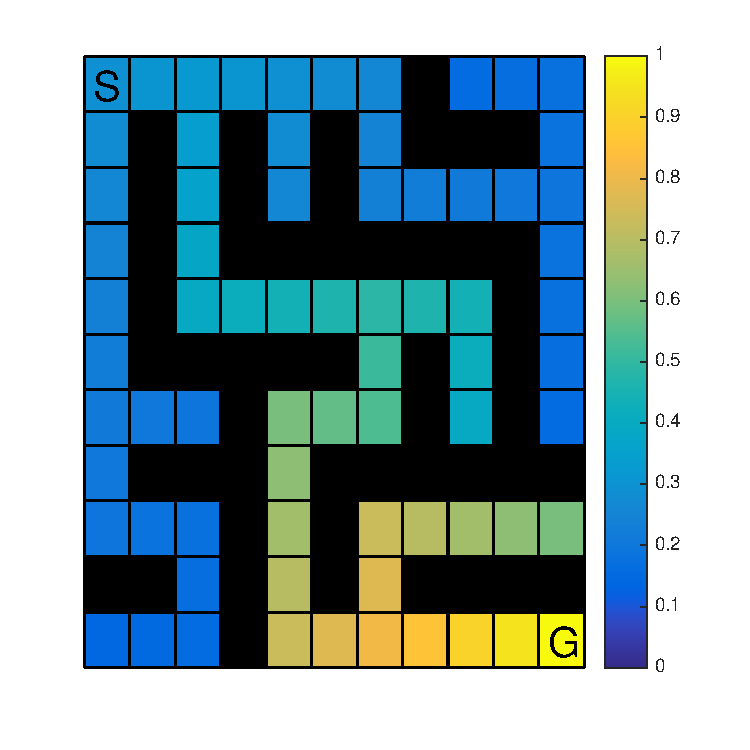
\includegraphics[width=0.5\textwidth]{maze_values}
\caption{Maze environment. Colors correspond to state values under the optimal policy, S is start state, and G is goal state.}
\label{fig:maze_values}
\end{figure}

\noindent
\textbf{Approximate pseudorewards} Dynamic programing was used to approximate state values by iterating over the Bellman equation. In~\cite{mcmahan2005bounded} conditions are defined under which initial state values will provably converge monotonically toward optimal values, but they note that in practice most reasonable initial values will achieve this monotonic convergence. Here, all states were initialized with a lower bound of zero and an upper bound of one, which, in our simple environment, is known to bound state values. Figure~\ref{fig:value_bounds} shows that the approximate state values for each state do indeed converge monotonically. The point at which each state reaches its optimal value is exactly equal to the minimum number of steps that state is from the goal. At each state, the pseudoreward for each action was calculated according to the shaping theorem as the difference between the value of the current state and the value of the of the next state given that action (which was deterministic in this environment). 

\begin{figure}[ht]
\centering
\includegraphics[width=0.45\textwidth]{value_bounds_labeled}
\caption{Monotonic convergence of estimated state values. Each subplot corresponds to a state in the maze. Red lines are upper bound estimate, blue lines lower bound estimate, and dashed lines optimal state values.}
\label{fig:value_bounds}
\end{figure}



\noindent
\textbf{Trading off model-free and model-based computation} The closer pseudorewards are to their optimal values, the easier the learning for the model-free agent (at least to some precision). However, whereas Q-learning is simple and quick, the model-based method of approximating state values is relatively slow and computationally costly. Therefore, we sought to understand the most efficient tradeoff between model-based pseudoreward approximation and model-free learning. This was done by computing the amount of CPU time (in seconds) required for each algorithm
%(while CPU time is a variable factor, the relative time across algorithms is generally invariant).

\subsection{Results}

Either the lower-bound of state values or the upper-bound after $n$ iterations of Bellman updates can be used to approximate pseudorewards for Q-learning, according to the shaping theorem. Figure~\ref{fig:maze1} shows the number of steps per episode needed to reach the goal, averaged across 50 episodes, as a function of the the number of Bellman updates used to approximate pseudorewards.
%The red line shows learning when approximate pseudorewards are based on upper-bound state values, and the blue line is for lower-bound values.
As expected, learning is quicker when pseudorewards are closer to their optimal values. For comparison, we also show performance of the Dyna algorithm, as a function of the number of planning steps taken after each real step.
%(separate horizontal axis in green).
While approximate pseudorewards are calculated just once using $n$ iterations, the planning steps used by Dyna are taken \textit{after every single step of every episode}.
%The dashed green lines show the number of real steps and the number of planning steps taken using Dyna.

Because Dyna must learn a model of the environment through experience, the first episodes require more than the minimal number of steps to learn the goal, which is why the average for real steps only is higher than the shortest path (34 steps when $\epsilon=0.25$). With sufficiently precise pseudorewards, on the other hand, the agent can learn the shortest path on the very first episode. Specifically, 24 Bellman updates are required for this, because the start state is 24 steps away from the goal state; after 24 iterations of the Bellman equation, optimal state values have propagated back from the goal state to the start state, along the shortest path.

Also shown are the number of steps taken by a simple Q-learning agent when states values are initialized to 0 (blue asterisk) or 1 (red asterisk).

\begin{figure}[ht]
\centering
\includegraphics[width=0.5\textwidth]{learning_vs_PRiterations_DYNA_mean}
\caption{Pseudoreward approximation requires fewer steps to reach the goal than Dyna. The number of steps taken to reach the goal, averaged across 50 episodes, is displayed as a function of the number of iterations of pseudoreward approximation, or the number of planning steps used by Dyna. With a sufficient number of iterations of pseudoreward approximation, the agent will reach the goal in the minimum number of steps on the very first episode.}
\label{fig:maze1}
\end{figure}

Next, we calculated the actual time (in CPU seconds) required to learn the shortest path. While the pseudoreward method may take fewer steps to reach the goal than Dyna, it does not necessarily mean that it is faster. Planning steps (which use scalar operations to update Q-values) are about two orders of magnitude quicker than Bellman updates (which require matrix multiplication), so it's possible that Dyna is still faster. However, Figure~\ref{fig:maze2} shows that pseudoreward approximation is still faster than Dyna. The fastest learning occurs when 24 iterations of the Bellman equation are used; any more than this is unnecessary and the CPU time gradually increases linearly.

\begin{figure}[ht]
\centering
\includegraphics[width=0.5\textwidth]{cpus_vs_PRiterations_DYNA_toGoal}
\caption{Pseudoreward approximation learns the shortest path more quickly than Dyna.}
\label{fig:maze2}
\end{figure}

\section{Experiment 2: Mountain car problem}

\subsection{Methods}

Experiment 2 explored learning in a classic mountain car environment~\cite{moore1990efficient, sutton1996generalization, sutton1998reinforcement, smart2000practical, rasmussen2003gaussian, whiteson2006evolutionary, heidrich2008variable, sutton2012dyna}. The agent begins in a valley between two mountains with the goal of reaching the top of the mountain on the right. The agent must learn to apply force such that it oscillates between the slopes of each mountain, building enough momentum until it finally reaches the top. States consisted of discretized locations along the 2-D mountainsides and discretized velocities. Actions consisted of discretized forces applied tangentially to the direction of movement. The agent used Q-learning during 200 learning episodes, where each episode ended when the car reached the goal state (or if 1,000 steps were taken). When the agent reached the goal it was conferred a reward of one (all other states had zero reward). An $\epsilon$-greedy decision policy was used where $\epsilon=0.01\times0.99^{i-1}$, where $i$ is the episode number. As before, all simulations were run one-hundred times and averaged together.

\noindent
\textbf{Comparison of learning methods} As before, pseudorewards were approximated using bounded dynamic programming and the shaping theorem. Performance using this algorithm was compared with Dyna.

\subsection{Results}

Figure~\ref{fig:mc1} shows the number of steps per episodes required to reach the goal, averaged across 200 episodes. Although not shown, the upper-bound and lower-bound estimates of state values all converged to optimal values after 73 iterations of the Bellman equation. 73 is the number of steps required to reach the goal from the starting state under the optimal policy, and thus after 73 Bellman updates, values from the goal state had propagated back to the start state (in this task the start state is the furthest possible state away from the goal).
%The x-axis shows the number of Bellman updates used to estimate pseudorewards. As before, the blue line indicates pseudorewards based on the lower-bound estimation of state values, and the red line is for the upper-bound approximation of state values. The green lines show the performance of Dyna.
The total number of steps (real steps plus simulated steps) far exceeds the number of steps using our method, and even the number of actual steps alone does not converge as low as the number of steps taken using our method.
%The blue asterisk indicates performance of a simple Q-learning agent.

\begin{figure}[t]
\centering
\includegraphics[width=0.5\textwidth]{MC_learning_vs_PRiterations_DYNA_mean}
\caption{Performance of the pseudoreward approximation method during the mountain car problem. The average number of steps taken across episodes is plotted against the number of model-based iterations of pseudoreward approximation. Also shown (green lines) is performance of Dyna.}
\label{fig:mc1}
\end{figure}

\begin{figure}[ht]
\centering
\includegraphics[width=0.5\textwidth]{MC_cpus_vs_PRiterations_DYNA_toGoal}
\caption{CPU time required to learn the shortest path.}
\label{fig:mc2}
\end{figure}

Figure~\ref{fig:mc2} shows the amount of time in CPU seconds required to learn the shortest path. Although Dyna requires many more steps to learn, because its computations are scalar-based Q-learning approximations, it is relatively quick, whereas Bellman approximation requires more costly matrix multiplication. Still, the pseudoreward approximation method learns more quickly.

\section{Discussion}

We have introduced a new method for cooperatively integrating model-free and model-based RL. This method relies on bounded dynamic programming to iteratively estimate state values that converge monotonically to values under the optimal policy. These approximate values are used to calculate pseudorewards according to the shaping theorem, such that the reward function is altered but the optimal policy is invariant. This reward function is used for model-free learning. Our experiments demonstrate that this method performs comparably and even better than the Dyna algorithm, a popular cooperative RL method.

\subsection{Equalizing knowledge}

One important difference between our method and Dyna is that Dyna learns the model of the environment, whereas our model is omniscient (that is, it is given the full state-action transition matrix and reward-action pairs). This may at first make any comparison between the two methods in terms of learning or computation time seem unfair. In actuality, however, if Dyna is given a full model so that it is equally omniscient, learning and and computation performance improves only modestly in the maze environment, and becomes worse in the mountain car task (these results are included in the Supplementary Material). An omniscient Dyna agent will only learn more quickly during the first episode, before it has discovered the location of reward. Once it knows how to reach the goal, a full model is unnecessary, and would even slow learning through planning, because unvisited states that do not help the agent reach the goal will be replayed, instead of focusing on useful states. One modification that would save computation time for Dyna would be to modulate the number of planning steps in proportion to the change in variance of estimated Q-values. When the temporal difference errors on average are larger, more planning steps are needed, but as they converge, the number of planning steps goes down.

\subsection{Learning the model}

Another way to make our method more comparable to Dyna is to have it learn its model. While our method is omniscient with respect to state-action transitions and rewards, this need not be the case. Our method can also be initialized with a naive model that has a uniform prior for all transition probabilities and reward outcomes (that is, any action is assumed to transition to any other state with equal probability and the expected reward for any action is $R/|{\cal S}|$, where $R$ is the expected reward for performing the task and $|{\cal S}|$ is the number of states in the environment). This model can be used for state value approximation with bounded RTDP, just as before, and as experience is acquired, the model can be updated (with either probabilistic transition estimates or deterministic ones if the environment is assumed to be such). When our method is run this way, it still outperforms Dyna in terms of steps required to learn, although it requires more CPU time since all planning steps use Bellman updates that require slow matrix multiplication (these results are also included in the Supplementary Material).

\subsection{Prioritized sweeping}

Another improvement to Dyna is known as prioritized sweeping~\cite{moore1993prioritized}. Here, the replay of state-action pairs is selected from the top of a queue, where the queue is sorted in descending order by the temporal difference error from that state-action pair. This allows states with the most uncertainty about their value to be replayed the most, and the effect of this is that learning of state values propagates backwards from rewarding states. If a prioritized sweeping algorithm were omniscient in the sense described above, then the number of planning steps needed to compute Q-values that would allow the agent to follow an optimal policy would simply be the distance from the start state to the goal state. While the number of real steps for prioritized sweeping is less that for Dyna, the number of planning steps is still very large, and the number of steps, either real or total, are still greater than for the pseudoreward agent. Moreover, sorting the queue after every simulated step, as described above, is extremely costly in terms of CPU time, and therefore takes much more CPU time to compute in practice (see the Supplementary Material for results).

\subsection{Pseudorewards and emotion}

By providing a new way to link model-free and model-based RL, our method offers a new way to think about human cognition, and to potentially test through experiments. While cooperative reinforcement learning in humans is only starting to be investigated behaviorally, there is substantial interest in understanding the interactions between them~\cite{daw2014algorithmic}. As discussed earlier, Dyna is readily likened to planning in human cognition as a means to train a model-free system. What might be an analog of pseudoreward approximation in human cognition? For any given task or goal-directed behavior, emotions quite often have the effect of altering the reward landscape, and it is reasonable to think of them as pseudorewards. If certain emotions represent the values of states that are stored in a model, and these emotions are used to train model-free learning by adding bonuses (positive emotions) or punishments (negative emotions) to certain actions, this would be quite akin to our method. The accuracy with which the emotion represents the value of a state would depend on the accuracy of the model, and could be implemented using Bellman approximation or something similar.

The method we have introduced links the two systems cooperatively by shaping the reward function. One way that this link may manifest in cognition is in the domain of moral decision making, where model-based production of emotions function as pseudorewards for model-free learning and decision making. It has been suggested that the dual-system approach to moral psychology is well described by the distinction between model-free and model-based RL, with the former describing the emotional, action-oriented system and the later mapping onto the rational, cognitive, and outcome-oriented system ~\cite{cushman2013action, crockett2013models}. Our method may provide a direct link between these two systems, with the model-based cognitive system producing particular emotions that function as pseudorewards, shaping the model-free emotional system. For example, when one's moral behavior deviates from one's understanding of ethics, leading to an untoward outcome, remorse could be generated to correct the action-oriented propensity that produced the misguided behavior. It is worth pursuing these questions experimentally to test the utility of our method for understanding human cognition and emotion.

\bibliography{model-free-model-based-shaping}{}
\bibliographystyle{apalike}

\end{document}
